\chapter{Raccolta dati ed implementazione}
\label{chap:implementazione}

Questo capitolo si occuperà, prima di tutto, di fornire dettagli sulle tecnologie e sulle modalità di raccolta dei dati da \textit{Twitter}, necessari alla costruzione di \textit{retweet graphs} associati ad \textit{hashtags} in \textit{input}.
\\Infine verrà trattata puntualmente l'implementazione degli algoritmi, definiti rigorosamente nel capitolo precedente, e di tutte quelle tecniche che hanno permesso di raggiungere l'obiettivo preposto, ovvero l'implementazione di un \textit{framework} che permetta di:
\begin{enumerate}
\item costruire ed analizzare \textit{retweet graphs} associati ad \textit{hashtags di Twitter} in \textit{input};
\item rilevare le \textit{echo-chambers} che caratterizzano la discussione;
\item eseguire un algoritmo di \textit{k-edge recommendation}, in modalità \textit{greedy} o meno;
\item fornire strumenti per l'analisi degli archi consigliati e per la visualizzazione dei nodi coinvolti (i.e. i nodi estremi degli archi consigliati).  
\end{enumerate}

\section{Raccolta dati}
La raccolta dei dati è una fase indispensabile, una condizione \textit{sine qua non}, senza la quale non è pensabile raggiungere alcun obiettivo tra quelli prefissati.
\\Poichè il \textit{software} proposto si occupa di \textit{endorsement graphs} della \textit{social network} di \textit{Twitter}, per la raccolta dei dati si è reso necessario l'utilizzo della \textit{Twitter Api}. Inoltre, visto che il linguaggio utilizzato per l'implementazione è \textit{Python}, sono state sfruttate le funzionalità della libreria \textit{Tweepy}, una via di accesso alla \textit{Twitter Api} di facile utilizzo. 
\\Nel seguito saranno forniti dettagli sugli strumenti di \textit{Twitter Api e Tweepy} e su altre tecniche che hanno permesso di \textit{bypassare} importanti limitazioni temporali delle \textit{Api di Twitter}.  

\subsection{Twitter Api}
\textit{Twitter} mette a disposizione degli sviluppatori delle \textit{Api}, utili per l'acquisizione dei dati pubblicati dagli utenti. Per rendere possibile il loro utilizzo bisogna innanzitutto creare un \textit{account Twitter} e poi effettuare l'iscrizione al \textit{reparto sviluppatori di Twitter}. Questa procedura è molto rigida e qualora non fosse seguita in modo rigoroso non sarebbe possibile utilizzare le \textit{Api}. 
\\Una volta effettuata l'iscrizione al \textit{reparto sviluppatori di Twitter}, è finalmente possibile procedere con la raccolta dei dati pubblicati dagli utenti, ma non prima di aver ottenuto le credenziali di accesso. Le credenziali vengono rilasciate a seguito della creazione di una \textit{Twitter App}, che rappresenta un \textit{progetto Twitter} dello sviluppatore: esse permetteranno di autenticarsi presso un \textit{server di Twitter}, con il quale sarà possibile interagire \textit{via streaming} mediante le \textit{Twitter Api} per ottenere i dati richiesti. Le credenziali si dividono in \textit{Token} e \textit{Consumer}, i quali hanno le seguenti caratteristiche e funzioni:
\begin{itemize}
\item il \textit{Token} permette l'accesso ai servizi che offre \textit{Twitter}. Non è sufficiente per consentire lo \textit{streaming} dei dati dal \textit{server}. \`E costituito da:
\begin{itemize}
\item \textit{Access Token};
\item \textit{Access Secret}.
\end{itemize}
\item il \textit{Consumer} consente lo \textit{streaming} dei dati di \textit{Twitter} dal \textit{server}. \`E costituito da:
\begin{itemize}
\item \textit{Consumer Key};
\item \textit{Consumer Secret}.
\end{itemize}
\end{itemize}
Nell'ambito della stessa \textit{Twitter App}, queste chiavi possono essere rigenerate a piacimento, anche con l'obiettivo di evitare problematiche relavite alla sicurezza. Qualunque sia il linguaggio di programmazione utilizzato per lo sviluppo del \textit{software} (nel caso in esame \textit{Python}), per utilizzare le \textit{Api} da codice è sempre necessario prima autenticarsi, fornendo tutti e quattro i codici appena elencati: le interfacce d'accesso alle \textit{Api} di \textit{Twitter} tuttavia dipendono dal linguaggio di programmazione e, nel nostro caso, sono realizzate mediante la libreria di \textit{Python Tweepy}, della quale parleremo nel seguito della trattazione.
\\Ad ogni modo, bisogna sottolineare che lo \textit{streaming} dei dati viene limitato da \textit{Twitter} per evitare che gli sviluppatori utilizzino in modo sconveniente i dati pubblicati dagli utenti: uno sviluppatore, pur essendo dotato di tutte le credenziali necessarie, non può effettuare più di 100 richieste ogni 15 minuti. Durante il tempo di pausa, che viene fatto scattare in corrispondenza del superamento della soglia di richieste, lo sviluppatore può decidere di aspettare che esso si esaurisca o, al contrario, può decidere deliberatamente di violarlo ed effettuare una nuova richiesta: in tal caso le sue credenziale verrebbero bloccate e non gli sarebbe permesso di comunicare con il \textit{server} mediante le \textit{Api} per circa un'ora.
\\Un'altra limitazione che impone l'\textit{Api} ufficiale di \textit{Twitter} riguarda l'impossibilità di ottenere \textit{tweets} più vecchi di una settimana: questa limitazione è molto forte ed ha costituito, nel processo di sviluppo del \textit{framework} proposto, un problema molto ingente, la cui risoluzione è dovuta alla libreria \textit{GetOldTweets di Python}, della quale parleremo presto.
\\Per terminare, i dati che lo sviluppatore richiede al \textit{server} mediante la \textit{Twitter Api} vengono restituiti in un file \textit{JSON}: esso conterrà tutti i \textit{metadati} necessari, i quali dipendono dal criterio della \textit{query}, come ad esempio il testo del \textit{tweet}, gli \textit{hashtags}, lo \textit{username} dell'utente che l'ha pubblicato e gli utenti che l'hanno \textit{retweettato}.

\subsection{Tweepy}
\textit{Tweepy} è una libreria di \textit{Python} che permette di accedere agevolmente alle \textit{Api} di \textit{Twitter}. Gestisce l'autenticazione dello sviluppatore presso il server di \textit{streaming} utilizzando i seguenti metodi:
\begin{enumerate}
\item \textit{tweepy.OAuthHandler(CONSUMER\_KEY, CONSUMER\_SECRET)}: 
\\una volta forniti \textit{Consumer Key e Consumer Secret} validi, restituisce un codice di autenticazione \textit{auth}; 
\item \textit{auth.set\_access\_token(ACCESS\_TOKEN, ACCESS\_TOKEN\_SECRET)}: 
\\permette di impostare il codice \textit{auth} con gli \textit{Access Token e Access Token Secret} (validi);
\item \textit{tweepy.API(auth)}: restituisce, in caso di corretta autenticazione, un oggetto \textit{Api} attraverso il quale può finalmente avvenire il processo di \textit{streaming} dal \textit{server}.
\end{enumerate}
Inoltre \textit{Tweepy} permette di gestire vari tipi di errore tra cui \textit{RateLimitError}, che insorge quando viene superata la soglia di traffico di 100 richieste ogni 15 minuti.

\subsection{GetOldTweets}
Come precedentemente detto, l'\textit{Api} ufficiale di \textit{Twitter} rende impossibile, con un semplice \textit{account} gratuito, l'acquisizione di \textit{tweets} più vecchi di una settimana. Questa limitazione, nel caso del sistema proposto, è intollerabile, visto che, per costruire \textit{retweet graphs} di dimensioni sufficienti a condurre un'analisi significativa, bisogna utilizzare un intervallo di osservazione abbastanza ampio. Superare tale limitazione continuando ad utilizzare l'\textit{Api} ufficiale vorrebbe dire pagare per ottenere un \textit{account Enterprise}, cosa che non siamo disposti a fare. 
\\La libreria \textit{GetOldTweets} permette di \textit{bypassare} l'\textit{Api} ufficiale e di ottenere \textit{tweets} più vecchi di una settimana semplicemente sfruttando la funzione \textit{scroll} della pagina di \textit{Twitter}: facendo \textit{scroll} verso il fondo pagina è possibile ottenere, tramite chiamate successive ad un \textit{provider JSON}, \textit{tweets} (relativi all'\textit{hashtag} che si sta cercando) via via più vecchi, evitando di incorrere a limitazioni temporali. Tale libreria mette a disposizione un gran numero di criteri di ricerca, utilizzati poi come parametri dell'indirizzo \textit{http}. Nel caso in esame sono stati utilizzati i seguenti parametri:
\begin{itemize}
\item \textit{Since}: una data limite inferiore per limitare la ricerca;
\item \textit{Until}: una data limite superiore per limitare la ricerca;
\item \textit{QuerySearch}: il testo di \textit{query} desiderato. Nel caso in esame, come \textit{query} viene sempre specificato un \textit{hashtag}, il quale identifica una discussione, e vengono considerati tutti e soli i \textit{tweets} creati nell'intervallo temporale specificato e che recano tale \textit{hashtag}.
\end{itemize}
Una volta costruito un oggetto \textit{tweetCriteria}, specificando le informazioni sopra elencate, esso viene passato come parametro al metodo \textit{getTweets} della classe \textit{TweetManager}, il quale si occupa di recuperare tutti i \textit{tweets} che soddisfano i criteri di ricerca. In particolare questo metodo, una volta costruita la \textit{url} contenente tutti i parametri di ricerca specificati, acquisisce la pagina \textit{web} contenente tutti i \textit{tweets} che soddisfano i criteri e converte il risultato in un formato \textit{JSON}. Le informazioni che, nel caso specifico dell'implementazione proposta, vengono estratte dai \textit{tweets} risultanti sono due:
\begin{itemize}
\item \textit{ID} del \textit{tweet};
\item \textit{Username} dell'autore del \textit{tweet}.
\end{itemize}
Gli \textit{ID} dei \textit{tweets} verranno utilizzati per recuperare tutti i \textit{retweets} associati, i quali sono indispensabili per costruire il \textit{retweet graph}.

\subsection{Flusso di esecuzione del processo di raccolta dati}

\begin{figure}
\begin{center}
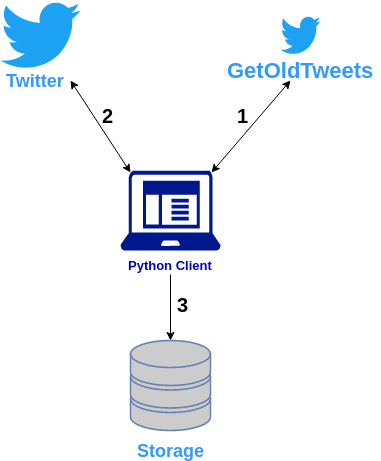
\includegraphics[scale=0.55]{images/raccolta_dati_tesi.png}
\end{center}
\caption{Processo di raccolta dati.}
\label{fig:raccolta_dati}
\end{figure}


\section{Implementazione}
